In this subsection the main characteristics of BERT will be outlined.

BERT, which stands for Bidirectional Encoder Representations from Transformers, is a new language representation model. Even if BERT was presented to the research world in May 2019, it has yet obtained new state-of-the-art results on eleven natural language processing tasks. For instance, a finetuned BERT push SQuAD v1.1 question answering F1 Test to 93.2 (1.5 points of absolute improvement) and SQuAD v2.0 F1 Test to 83.1 (5.1 points of absolute improvement) \cite{bert}.

The training framework proposed by the authors of BERT is composed of two steps:
\begin{enumerate}
  \item \textit{pre-training}: BERT is trained over different pre-training tasks.
  \item \textit{fine-tuning} over a single downstream task: in this case, the SQuAD task.
\end{enumerate}

BERT’s  model  architecture is a multi-layer bidirectional Transformer encoder. These last components, that are the building blocks of BERT, are implemented as described in \cite{attentionisallyouneed}.

Considering BERT Base, the size taken in consideration for this project, the hidden layers (i.e. Transformers encoders) are $12$, the hidden size is $768$ and the number of self-attention heads is $12$.

\begin{figure}[t]
\centering
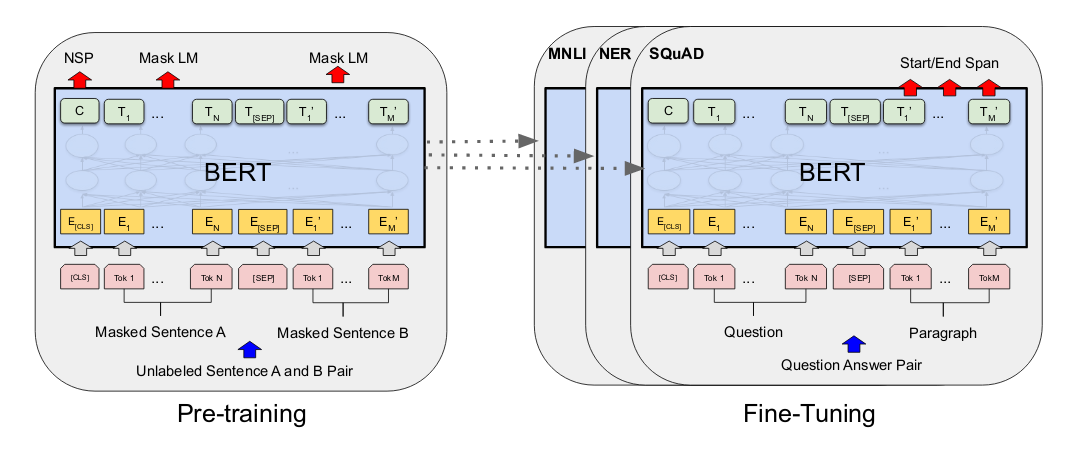
\includegraphics[width=18cm]{bert-for-squad-original-paper}
\caption{Overall pre-training and fine-tuning procedures for BERT. The pre-training procedure provides a basis for the numerous possible downstream tasks. \texttt{[CLS]}, which stands for ``classification'', is a special symbol added in front of every input example, and \texttt{[SEP]} is a special separator token. For further information about the input representation, see \cite{bert}. Image taken from \cite{bert}.}
\medskip
\label{fig:bertsquad}
\end{figure}

\subsubsection{Pre-training BERT}
Briefly, pre-training BERT means training it on two tasks:
\begin{itemize}
  \item \textit{Masked Language Model} (MLM), often called \textit{Cloze task}. A bidirectional model like BERT is undoubtedly more powerful than a left-context model like the OpenAI GPT Transformer. But this type of model is even more difficult to train because a bidirectional conditional language model cannot be trained left-to-right or right-to-left, since this would allow each word to indirectly ``see itself'' during training.

  Thus, in order to train a bidirectional representation, the researchers simply mask some percentage of the input tokens at random (15\% in their experiments), and then predict those masked tokens. This means substituting a real token with a placeholder token \texttt{[MASK]}.
  
  \item \textit{Next Sentence Prediction} (NSP). This task is beneficial to many important downstream tasks like Question Answering and Natural Language Inference that are based on understanding the relation between two sentences, skill that is not captured by the previous task. Basically, it is a binary \textit{next sentence prediction}: when choosing the sentences \texttt{A} and \texttt{B} for the training, in the 50\% of the cases \texttt{B} is an actual next sentence of \texttt{A} (and it is labeled as \texttt{IsNext}) while in the other cases the choice of \texttt{B} is random between the sentences (labeled as \texttt{NotNext}).
\end{itemize}

\subsubsection{A dataset for Reading Comprehension: SQuAD}
\label{squad}
In the fine-tuning stage BERT is trained on SQuAD, a dataset for Reading Comprehension developed by Stanford University \cite{squad}. It consists in a collection of $100\,000$ question-answer pairs over different Wikipedia passages. There are two versions of SQuAD: the first version (\texttt{v1.1}) contains only questions over a passage that have an answer, while the second version (\texttt{v2.0}) has some questions without answer. Obviously, doing better on SQuAD 2.0 is more difficult, because it requires a minimum level of reasoning.

\subsubsection{Fine-tuning BERT on SQuAD1.1}
As illustrated in Figure \ref{fig:bertsquad}, during fine-tuning passage and question are both passed to BERT (separated by the \texttt{[SEP]} tag). This phase introduces two trainable vectors: $S$ (for the start of the answer) and $E$ (for the end of the answer) both of dimension $\mathbb{R}^\mathbb{H}$ ($\mathbb{H}$ is the hidden size, $768$ for BERT Base). 

The probability of a token $i$ of being the start of the answer is:
\begin{equation}
P_{i} = \frac{\mathrm{e}^{S \cdot T_{i}}}{\sum_{j} \mathrm{e}^{S \cdot T_{j}}}
\end{equation}
where $T$ is the last layer of BERT. The analogous formula is used for the end of the answer.

The score of a candidate span that goes from token $i$ to token $j$ is defined as:
\begin{equation}
\text{score}_{i, j} = S \cdot T_{i} + E \cdot T_{j}
\end{equation}

The maximum score is reached where $j \geq i$ is used as prediction.

Finally, the training objective is defined as the sum of the two log-likelihoods \eqref{eqn:loglikelihood} of the correct start and end positions.

\begin{equation}
\label{eqn:loglikelihood}
\text{loglikelihood}(S) = \sum_{i} y_{i} \mathrm{ln} (P(y_{i} | S)) + (1 - y_{i}) \mathrm{ln} (1 - P(y_{i} | S))
\end{equation}

For the purpose of this work, the pretrained BERT-SQuAD model by DeepPavlov \cite{deeppavlov} was used.
